% !TeX document-id = {38ad272c-6b95-4178-b409-8ae7f3766667}
% !TeX spellcheck = en_US
% !TeX root = ../../build/architecture.tex
% !TeX TXS-program:compile = txs:///xelatex/[--shell-escape]


\renewcommand{\mytitle}{Layer 2 Scalability Strategies}
\ifZEROSEC \fi
\ifSEC \section{\mytitle{}}\fi
\ifSUBSEC \subsection{\mytitle{}}\fi
\ifSUBSUBSEC \subsubsection{\mytitle{}}\fi


\begin{frame}{Building a Layer 2}
\begin{columns}
\begin{column}{0.35\textwidth}
\begin{itemize}
\item Let's assume that our layer 2 is called x ($L2_x$).
\item The state of the layer x progresses with its L2 transactions.
\end{itemize}
\end{column}
\begin{column}{0.65\textwidth}
\begin{figure}
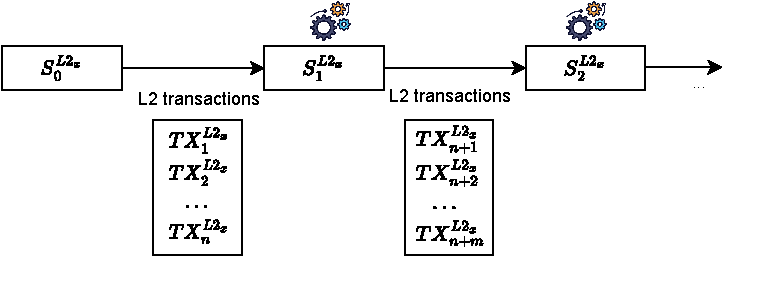
\includegraphics[width=\columnwidth]{\zkevmdir/figures/concepts/l2-scaling-strategies/l2-state.drawio}
\end{figure}
\end{column}
\end{columns}

\begin{itemize}
\item There are many questions to answer to build an L2:
  \begin{enumerate}[a)]
  \item How users send L2 transactions and who receives them?
  \item How these L2 transactions are made publicly available (if so)?
  \item Who processes the L2 transactions and how, and, when 
  it is publicly considered that a new state is correctly computed?
  \item What type of applications the L2 supports? simple or rich processing?
  \end{enumerate}
\end{itemize}
\end{frame}




\begin{frame}{Layer 2 Design: Sending L2 Transactions}
\textbf{Q.} How users send L2 transactions and who receives them?
  \begin{itemize}
  \item \textbf{Unicast}: an unicast communication with some (centralized) entity.
  \item \textbf{Peer-to-peer}: a peer-to-peer network where everybody (decentralized) receives the L2 transactions.
  \item \textbf{Smart contract}: a smart contract in the L1 execution layer (decentralized).
  \end{itemize}

\vspace{1em}

\begin{columns}[t]

\begin{column}{0.3 \textwidth}
\centering
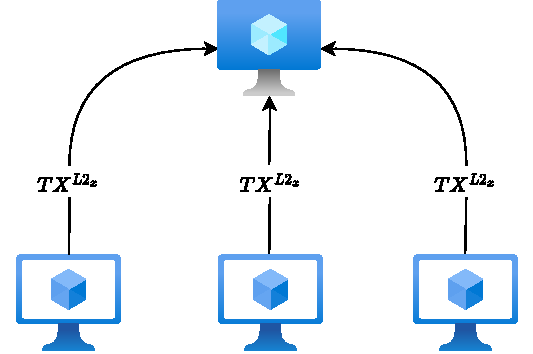
\includegraphics[width=.8\columnwidth]{\zkevmdir/figures/concepts/l2-scaling-strategies/unicast.drawio}
\textbf{Unicast}
\end{column}

\begin{column}{0.3 \textwidth}
\centering
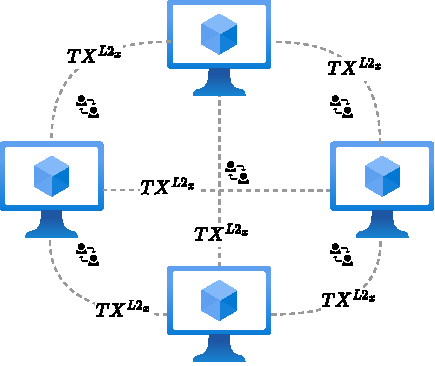
\includegraphics[width=.8\columnwidth]{\zkevmdir/figures/concepts/l2-scaling-strategies/peer-to-peer.drawio}
\textbf{Peer-to-Peer}
\end{column}

\begin{column}{0.3 \textwidth}
\centering
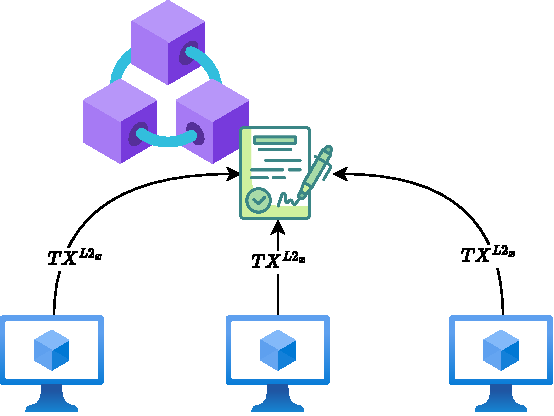
\includegraphics[width=.8\columnwidth]{\zkevmdir/figures/concepts/l2-scaling-strategies/sc-l2-tx.drawio}
\textbf{Smart Contract}
\end{column}

\end{columns}

\end{frame}




\begin{frame}{Layer 2 Design: L2 Data Availability}
\textbf{Q.} How are L2 transactions made publicly available (if so)?
\begin{itemize}
\item To achieve L2 data availability in Ethereum, currently, we can proceed in two ways:
  \begin{itemize}
  \item As a \textbf{validium} in which L2 data is managed by a group of \textbf{trusted} entities (\textbf{data managers}), being
  this approach far more \textbf{cheaper} than writing to L1.
  \item As a \textbf{rollup}, which writes L2 data in the public L1 Execution layer, meaning that the posted data will be publicly available.
  \end{itemize}
\item In the future, with the introduction of the EIP-4844, a third option opens up with \textbf{data shards}.
\end{itemize}
\end{frame}


\begin{frame}{L2 Rollups}
\begin{columns}
\begin{column}{0.65\textwidth}
\begin{figure}
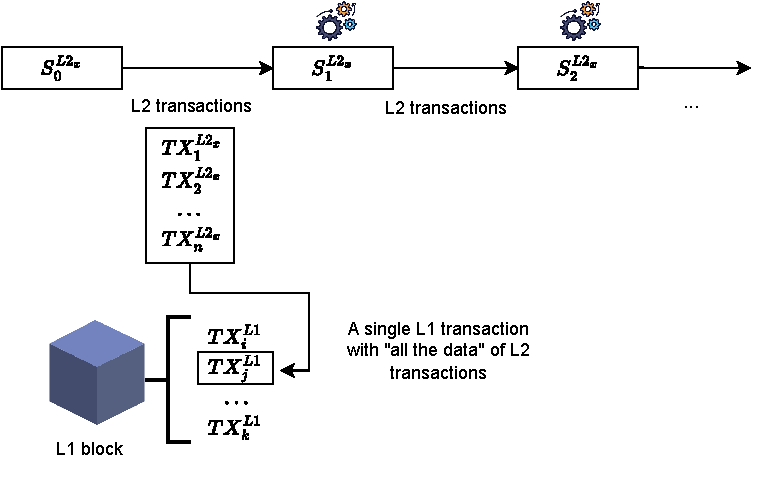
\includegraphics[width=\columnwidth]{\zkevmdir/figures/concepts/l2-scaling-strategies/l2-rollup.drawio}
\end{figure}
\end{column}

\begin{column}{0.35\textwidth}
\begin{itemize}
\item In this case, to provide data availability, we use a single L1 transaction that contains a batch of L2 transactions.
\item This idea is also called a \textbf{rollup}, because we "roll up" a bunch of L2 transactions in a single L1 transaction.
\end{itemize}
\end{column}
\end{columns}
\end{frame}

\begin{frame}{L2 Validiums}
\begin{columns}
\begin{column}{0.65\textwidth}
\begin{figure}
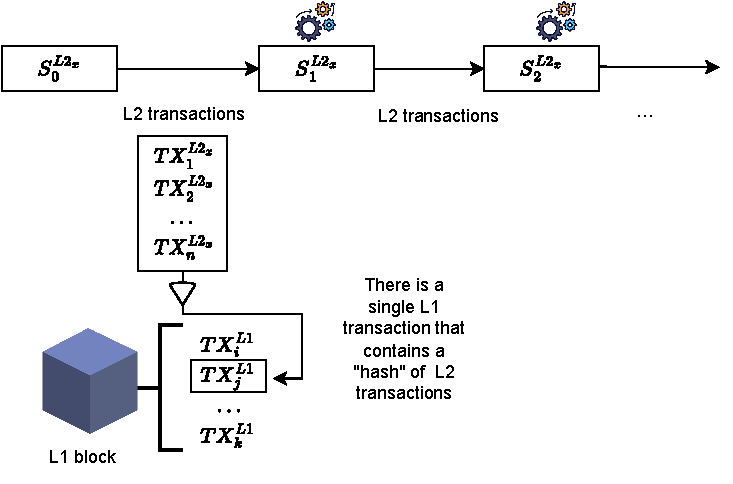
\includegraphics[width=0.9\columnwidth]{\zkevmdir/figures/concepts/l2-scaling-strategies/l2-validium.drawio}
\end{figure}
\end{column}
\begin{column}{0.35\textwidth}
  In a validium, the L1 transaction only includes a cryptographic summary of the L2 transactions.
\end{column}
\end{columns}
\end{frame}


\begin{frame}{Layer 2 Design: State Computation}
\textbf{Q.} Who processes the L2 transactions and how, and, when it is publicly considered that a new state is correctly computed?
\begin{itemize}
\item Recall that we need to compute the next L2 state $S^{L2_x}_{i+1}$ from a set of $L2^x$ transactions and the current state $S^{L2_x}_i$.
\item We can do that in several ways:
  \begin{enumerate}[a)]
  \item Centralized execution.
  \item Optimistic execution.
  \item Succinct computation verification (zk technology).
  \end{enumerate}
\end{itemize}
\end{frame}






\begin{frame}{Centralized Execution}
\begin{columns}
\begin{column}{0.6\textwidth}
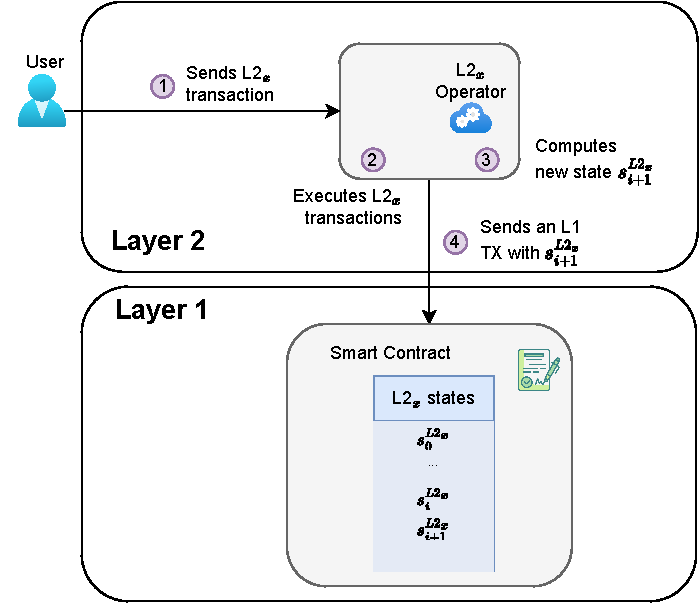
\includegraphics[width=0.9\columnwidth]{\zkevmdir/figures/concepts/l2-scaling-strategies/l2-centralized-design.drawio}
\end{column}
\begin{column}{0.4\textwidth}
\begin{itemize}
\item In this approach, the state computation is considered final quickly (takes only "seconds or minutes").
\item However, this approach has the issue of how ``we" (as external entities) dispute the L2 operator
about the correctness of an L2 state computation?
\end{itemize}
\end{column}
\end{columns}
\end{frame}





\begin{frame}{Optimistic Execution}
\begin{columns}
\begin{column}{0.45\textwidth}
\begin{itemize}
\small
\item An \textbf{Optimistic L2} provides a decentralized execution mechanism that allows
disputing the correctness of the L2 state computation.
\item With this approach, there is a (large) period of time to allow
anybody to send a \textbf{fraud proof},
proving that the state was wrongly computed (for example, a double spending transaction).
\end{itemize}
\end{column}
\begin{column}{0.53\textwidth}
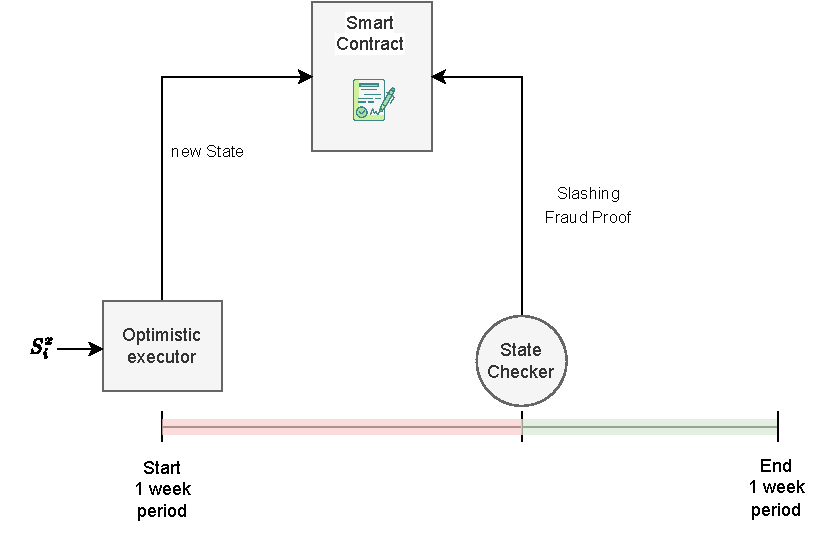
\includegraphics[width=0.93\columnwidth]{\zkevmdir/figures/concepts/l2-scaling-strategies/optimistic-fraud-proof.drawio}
\end{column}
\end{columns}
\begin{itemize}
\small
\item If the Optimistic Executor does its job correctly,
 it will earn ETH.
\item Otherwise, executor is slashed and \textbf{state checker} is rewarded 
(for providing the fraud proof).
\item Notice that the progress of the state with optimistic execution is slow,
since in general, it takes "days" to consider the state as final.
\end{itemize}
\end{frame}





\begin{frame}[t]{Succinct Execution Verification (zk* Systems)}
\begin{itemize}
\small
\item In the succinct execution verification model, instead of an optimistic executor,
we have an execution \textbf{prover}.
\item The prover can prove that an execution of a set of L2 transaction is correct.
\item The set of L2 transactions being proved is called a \textbf{batch}.
\item The prover uses \textbf{Zero-Knowledge (ZK)} technology.
\end{itemize}

\begin{columns}
\begin{column}{0.4\textwidth}
\centering
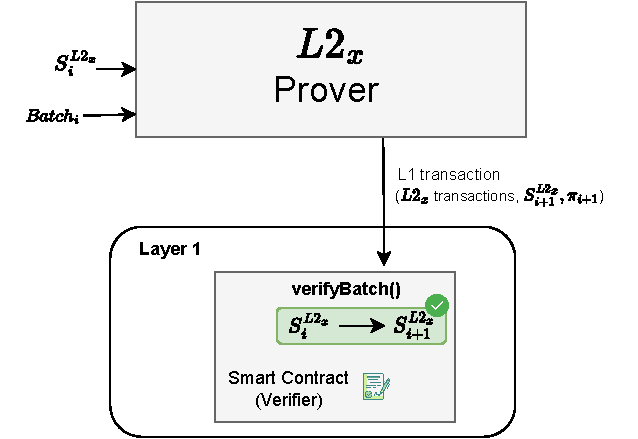
\includegraphics[width=0.9\columnwidth]{\zkevmdir/figures/concepts/l2-scaling-strategies/succinct-execution-prover-verifier.drawio}
\end{column}
\begin{column}{0.6\textwidth}
\begin{itemize}
\small
\item A smart contract in L1 is the \textbf{verifier} of the proof of the batch execution.
\item There is no possible dispute since the ZK proof proves that state is correctly computed.
\item When the smart contract executes the transaction, we say that the next state, $S^x_{i+1}$, is \textbf{consolidated}.
\item With this approach, the state computation is quickly considered final since
it takes only "seconds or minutes" to generate and validate the proof.
\end{itemize}
\end{column}
\end{columns}
\end{frame}






\begin{frame}[t]{Remarks about Prover and Verifier}
\begin{columns}
\begin{column}{0.55\textwidth}
\begin{itemize}
\item Regarding the \textbf{prover}:
  \begin{itemize}
  \item It is typically allocated in a cloud service.
  \item Uses a considerable amount of resources (mainly RAM and CPU).
  \end{itemize}

\vspace{0.2cm}
\item Regarding the \textbf{verifier}:
  \begin{itemize}
  \item The proof size is small

  (just a few bytes).
  \item The verification time is also small

  (of the order of $\mu$s).
  \item As a result, a smart contract can indeed verify proofs of L2 batch processing.
  \end{itemize}
\end{itemize}
\end{column}
\begin{column}{0.4\textwidth}
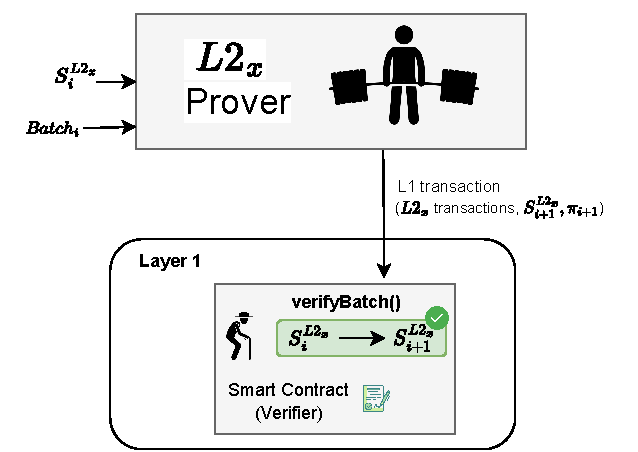
\includegraphics[width=0.95\columnwidth]{\zkevmdir/figures/concepts/l2-scaling-strategies/succinct-execution-powers.drawio}
\end{column}
\end{columns}
\end{frame}




\begin{frame}[t]{Summary of the L2 Scaling Solutions}
Scalability solutions for blockchains can be classified by two main dimensions:
  \begin{itemize}
  \item \textbf{Data availability.} Whether the data from the L2 chain is available on-chain (in L1) or off-chain (only in the L2 chain).
  \item \textbf{Mechanism to state correctness.} How the correctness of the L2 chain is guaranteed.
  \end{itemize}

\vspace{0.35cm}
\begin{figure}
\begin{tabular}{|c|c|c|}
\hline
\cellcolor{darkgray} & \cellcolor{darkgray} \color{white} Validity Proof  & \cellcolor{darkgray} \color{white} Fraud Proof \\ \hline
\cellcolor{lightgray} Data on-chain   & zkRollup       & Optimistic Rollup \\ \hline
\cellcolor{lightgray} Data off-chain  & zkValidium     & Plasma \\ \hline
\end{tabular}
\end{figure}

\centering
\vspace{0.2cm}
\url{https://l2beat.com/scaling/summary}
\end{frame}




% \begin{frame}[allowframebreaks]{Remarks about zkValidiums}
% \begin{columns}
% \begin{column}{0.35 \textwidth}
% \begin{itemize}
% \small
% \item In \textbf{zkValidium}, instead of posting all the batch data back to L1, only a cryptographic summary (a \textit{hash}) of it is posted.
% \item This means that a user cannot retrieve the L2 transactions from L1. 
% \item Instead, the user must ask a \textit{reliable} L2 operator (data manager) for these data.
% \end{itemize}
% \end{column}
% \begin{column}{0.65 \textwidth}
% \begin{figure}
% \centering
% 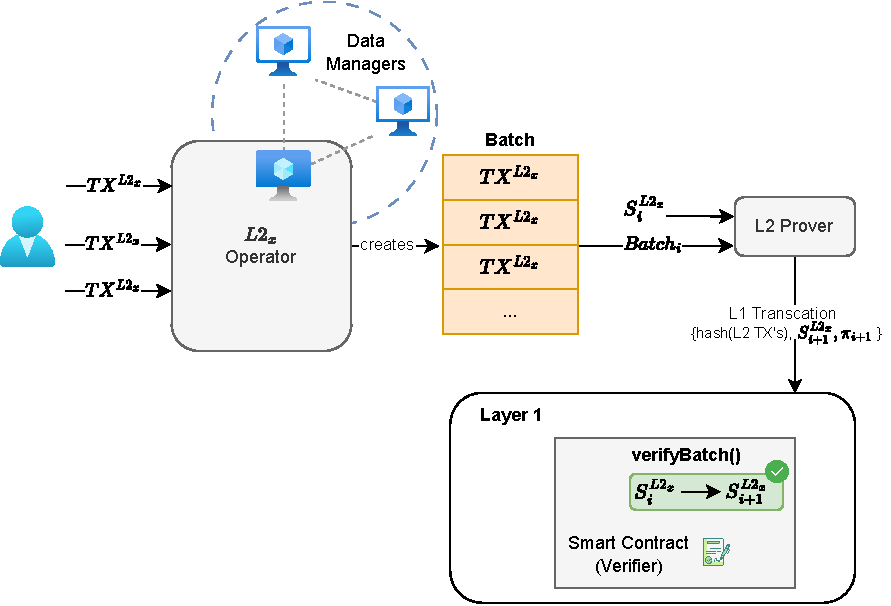
\includegraphics[width=\columnwidth]{\zkevmdir/figures/concepts/l2-scaling-strategies/validium.drawio}
% \end{figure}
% \end{column}
% \end{columns}

% \framebreak
% In case the operators do not provide the data to the user, still the ZK processing assures that the transactions included in the batch
% are always correctly processed.

% \vspace{0.2cm}
% This means that, for example: 

% \vspace{0.1cm}
%   \begin{itemize}
%   \item No one can steal your funds. 
%   \item You might see an increase in your L2 balance, but you might not know which concrete L2 transaction produced this increase.
%   \end{itemize}
% \end{frame}






\begin{frame}{L2 Applications: Simple or Rich Processing}
\begin{figure}
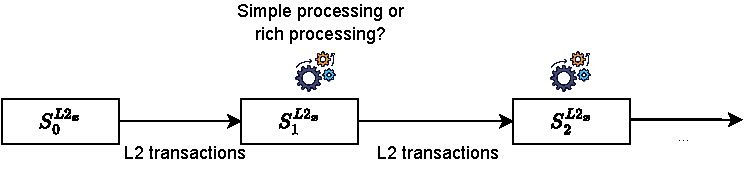
\includegraphics[width=0.6\columnwidth]{\zkevmdir/figures/concepts/l2-scaling-strategies/l2-applications.drawio}
\end{figure}

\textbf{Q.} What type of applications the L2 supports?
\begin{itemize}
\item \textbf{Simple asset transfers}, e.g. tokens or payment network with "simple processing" of the transactions.
\item \textbf{General purpose execution virtual machine}, e.g. EVM with "rich processing" of the transactions.
\end{itemize}
\end{frame}





\begin{frame}{L2 Simple Processing}
\begin{figure}
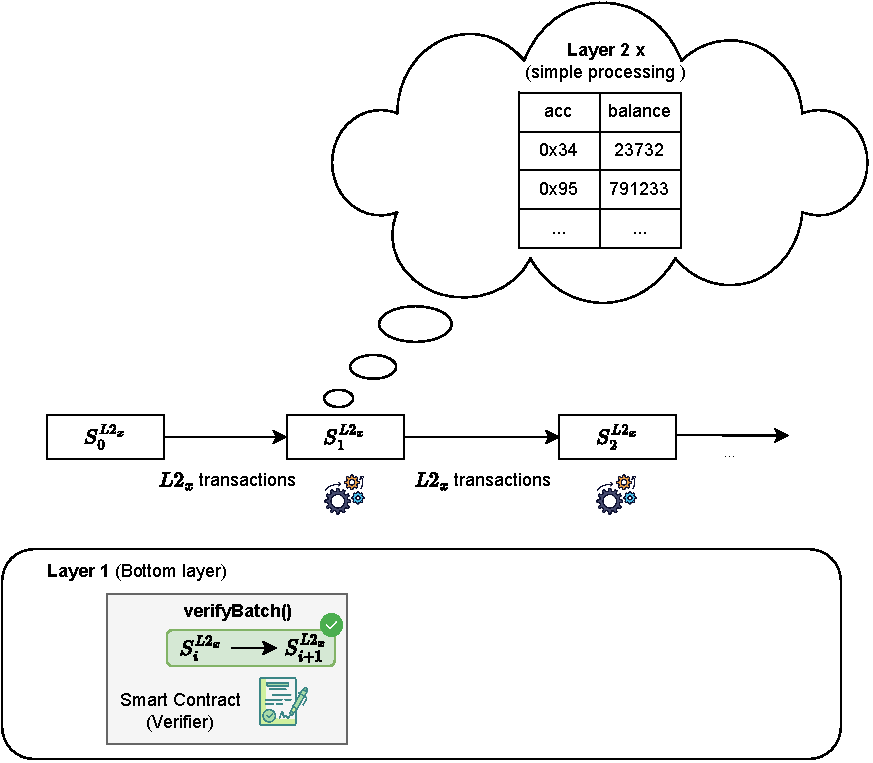
\includegraphics[width=0.53\columnwidth]{\zkevmdir/figures/concepts/l2-scaling-strategies/l2-simple-processing.drawio}
\end{figure}
\end{frame}






\begin{frame}{L2 Rich Processing (zkEVM)}
\begin{figure}
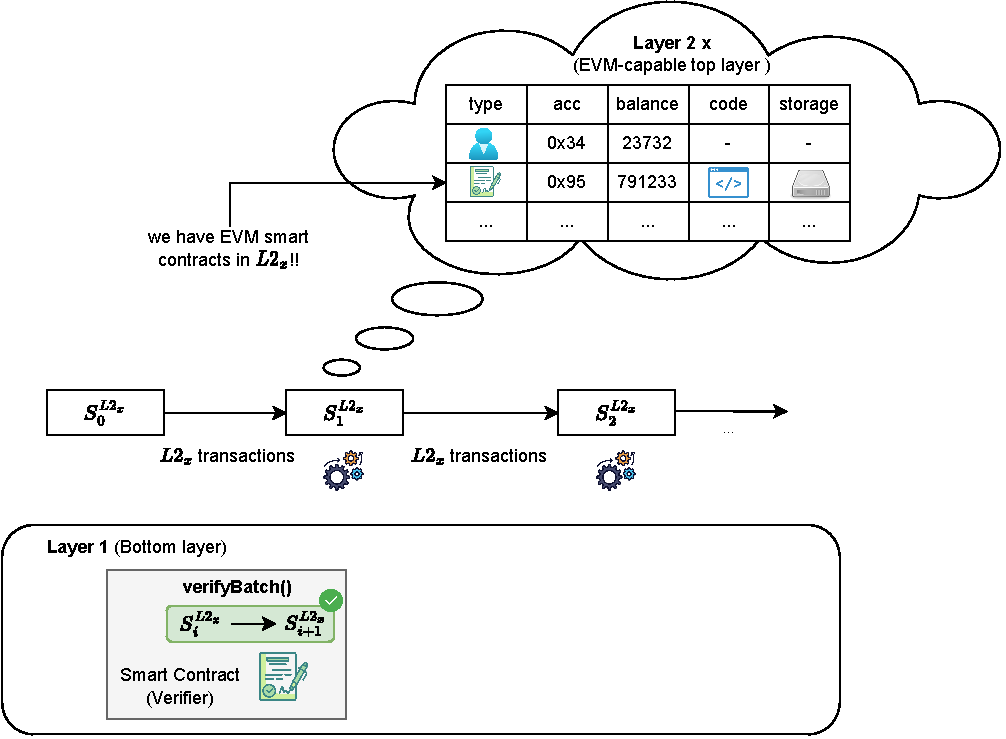
\includegraphics[width=0.6\columnwidth]{\zkevmdir/figures/concepts/l2-scaling-strategies/l2-rich-processing-zkevm.drawio}
\end{figure}
\end{frame}



\begin{frame}[fragile, allowframebreaks]{zkEVMs Compatibility/Equivalence}
\begin{figure}
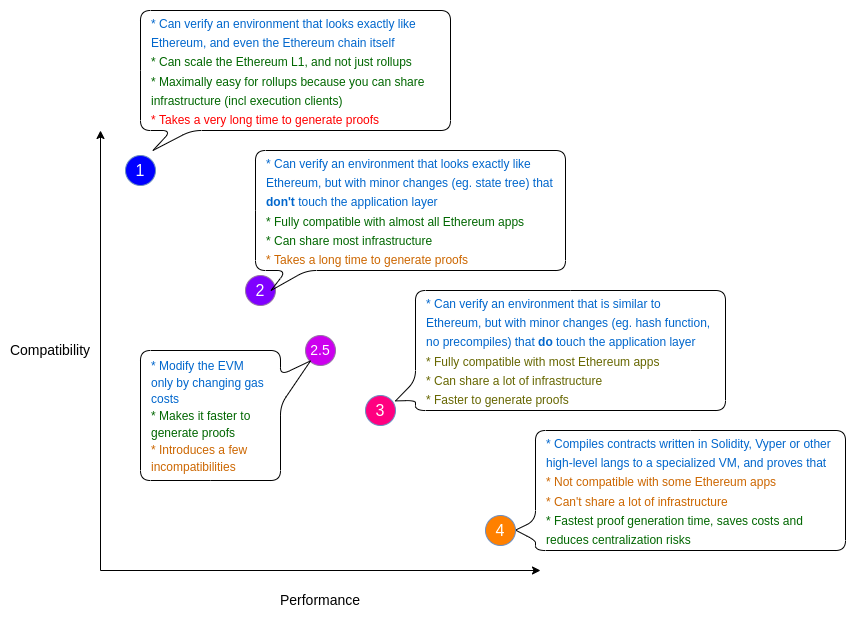
\includegraphics[width=0.6\columnwidth]{\zkevmdir/figures/architecture/intro-proving-system/zkEVM-compatibility-post-vitalik}
\end{figure}
\end{frame}




\begin{frame}{Are we Scaling with zkRollups?}
\ifPROF
\footnotesize
\textbf{++Prof:} This is a natural question since all the L2 data is somehow posted in the L1 chain.
\normalsize
\fi

\textbf{Q.} A last natural question is if we are scaling with rollups based on succinct verification.

\textbf{The answer is yes}, because the smart contract execution resources for verifying a proof are much lower
than executing individual transactions within a batch.


In fact, the majority of the cost comes from the data availability, but we can work on improve the costs of data availability.

\vspace{0.2cm}
Addressing data availability costs:
  \begin{itemize}
  \item Succinct verification of \textbf{compressed} data (for example, transaction digital signature).
  \item EIP 4844 \textbf{Proto-Danksharing}:
    \begin{itemize}
    \item Data shards are much cheaper than writing in L1 execution layer.
    \item Remark that the L1 execution layer (smart contracts) will have access to blobs in data shards.
    \end{itemize}
  \end{itemize}
\end{frame}
